\documentclass[11pt,a4paper]{article}
\usepackage[T1]{fontenc}
\usepackage[utf8]{inputenc}
\usepackage{lmodern}
\usepackage[margin=2cm]{geometry}
\usepackage{microtype}
\usepackage{enumitem}
\usepackage{tabularx}
\usepackage{booktabs}
\usepackage{titlesec}
\usepackage{xurl}
\usepackage[hidelinks]{hyperref}
\usepackage{tikz}
\usetikzlibrary{positioning,arrows.meta}

\setlength{\parindent}{0pt}
\setlength{\parskip}{5pt}
\setlist{nosep,leftmargin=*,topsep=2pt}
\titleformat{\section}{\large\bfseries}{\thesection}{0.6em}{}
\titlespacing*{\section}{0pt}{9pt}{3pt}

\tikzset{
  box/.style={draw,rounded corners=2pt,align=center,font=\small\ttfamily,inner sep=4pt,minimum height=7mm},
  ext/.style={box,fill=gray!12,font=\small},
  lbl/.style={font=\scriptsize,midway},
  arr/.style={-{Stealth[length=2mm]},thick}
}

\begin{document}

{\LARGE\bfseries Crypto \& Stock Alerts Telegram Bot}\par
\vspace{2pt}
{\large\itshape DevOps project report}\par
\vspace{2pt}
{\large Jafar (\href{mailto:jafarm@kth.se}{jafarm@kth.se}) and Gabriel (\href{mailto:gaag2@kth.se}{gabo26126@outlook.com})}\par

\section{Project and architecture}

We built a Telegram bot that lets users set price alerts for cryptocurrencies and stocks. Users subscribe with \texttt{/subscribe}, review alerts with \texttt{/list} and remove them with \texttt{/unsubscribe}; a background scheduler polls market prices and messages the user the moment a target is hit. We scoped the application deliberately so the engineering effort could go into the DevOps workflow around it: CI, CD, Infrastructure as Code, and automated quality and security checks. The application, tests, container configuration, workflows, Terraform and documentation all live in one GitHub repository, so a single pull request can change and review any of them together.

\begin{figure}[h]
\centering
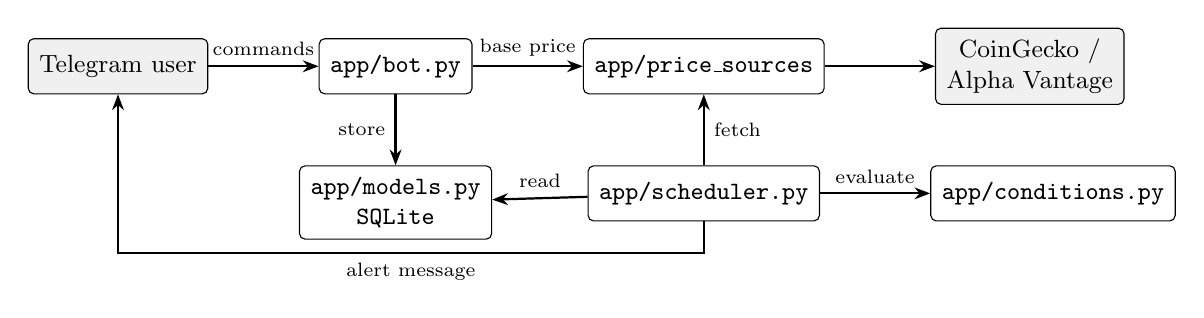
\begin{tikzpicture}[node distance=5mm and 14mm]
  \node[ext] (user) {Telegram user};
  \node[box,right=of user] (bot) {app/bot.py};
  \node[box,right=of bot] (src) {app/price\_sources};
  \node[ext,right=of src] (apis) {CoinGecko /\\Alpha Vantage};
  \node[box,below=9mm of bot] (models) {app/models.py\\SQLite};
  \node[box,below=9mm of src] (sched) {app/scheduler.py};
  \node[box,right=of sched] (cond) {app/conditions.py};
  \draw[arr] (user) -- node[lbl,above]{commands} (bot);
  \draw[arr] (bot) -- node[lbl,above]{base price} (src);
  \draw[arr] (src) -- (apis);
  \draw[arr] (bot) -- node[lbl,left]{store} (models);
  \draw[arr] (sched) -- node[lbl,above]{read} (models);
  \draw[arr] (sched) -- node[lbl,right]{fetch} (src);
  \draw[arr] (sched) -- node[lbl,above]{evaluate} (cond);
  \draw[arr] (sched.south) -- ++(0,-4mm) -| node[lbl,pos=0.25,below]{alert message} (user.south);
\end{tikzpicture}
\caption{Application components and how they interact.}
\end{figure}

\texttt{app/main.py} wires configuration, the database, the command handlers and the scheduler together. The two price providers sit behind one \texttt{get\_price(symbol)} interface, and \texttt{app/conditions.py} holds pure trigger logic with no network or database access. We chose this separation because it keeps external I/O at clear boundaries and makes the core logic easy to unit-test. Long polling means the bot needs no public endpoint, and SQLite avoids running a separate database server for a single process.

\section{Development platform and continuous integration}

GitHub is our development platform: source control, pull requests, branch rules, Actions, security results and the container registry (GHCR) all live there. We work on feature branches and merge through pull requests. A ruleset on \texttt{main} requires a pull request, one approving review, and passing \texttt{lint}, \texttt{test} and \texttt{docker-build} checks. Force pushes and deletion are blocked and the bypass list is empty, so no change lands just because it compiles locally or because one person wrote it.

The CI workflow runs on every push and pull request with five jobs:
\begin{itemize}
  \item \textbf{lint} runs Ruff. One tool covers style, import order, modernization and common bug patterns, instead of several separate linters.
  \item \textbf{test} runs pytest over the trigger logic, persistence layer and price sources, with external HTTP calls mocked so the job doesn't depend on third-party availability or rate limits. It fails if coverage drops below 40\%, a floor set just under the current figure.
  \item \textbf{integration-test} calls the real Telegram Bot API to check that a valid token is accepted and an invalid one is rejected, which catches a revoked token or an API change that mocks can't. The tests skip when the token secret is missing, as on a fork's pull request, and the job is \texttt{continue-on-error}, so merges and deploys go ahead even when Telegram is down.
  \item \textbf{docker-build} builds the production image, catching broken Dockerfiles or missing dependencies before merge.
  \item \textbf{secret-scan} runs Gitleaks, pinned to v8.30.1 so CI only picks up a new version when we bump it, and fails when it finds a committed secret.
\end{itemize}
A separate CodeQL workflow runs static security analysis on pull requests to \texttt{main} and once a week. Figure~\ref{fig:pipeline} shows how these checks connect to delivery.

\begin{figure}[h]
\centering
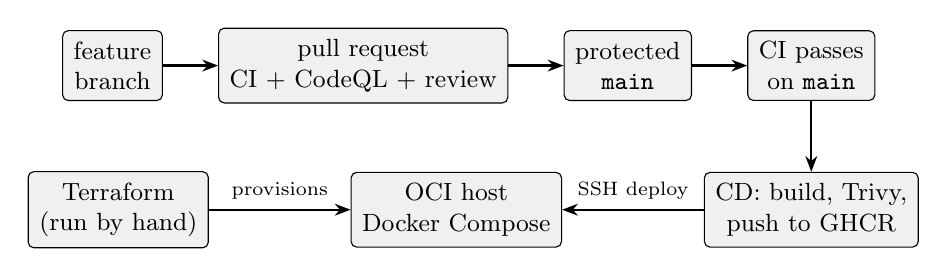
\begin{tikzpicture}[node distance=5mm and 7mm]
  \node[ext] (branch) {feature\\branch};
  \node[ext,right=of branch] (pr) {pull request\\CI + CodeQL + review};
  \node[ext,right=of pr] (main) {protected\\\texttt{main}};
  \node[ext,right=of main] (ci) {CI passes\\on \texttt{main}};
  \node[ext,below=9mm of ci] (cd) {CD: build, Trivy,\\push to GHCR};
  \node[ext,left=18mm of cd] (host) {OCI host\\Docker Compose};
  \node[ext,left=18mm of host] (tf) {Terraform\\(run by hand)};
  \draw[arr] (branch) -- (pr);
  \draw[arr] (pr) -- (main);
  \draw[arr] (main) -- (ci);
  \draw[arr] (ci) -- (cd);
  \draw[arr] (cd) -- node[lbl,above]{SSH deploy} (host);
  \draw[arr] (tf) -- node[lbl,above]{provisions} (host);
\end{tikzpicture}
\caption{From a feature branch to a running deployment.}
\label{fig:pipeline}
\end{figure}

\section{Continuous delivery and containerization}

The CD workflow starts only after CI succeeds on \texttt{main}, and it builds and deploys the commit CI tested. Deploys run one at a time, so two quick merges can't race on the host. The image is tagged with the commit SHA and \texttt{latest}; the SHA tag ties each deployed image to the source revision that produced it.

Trivy scans the image for HIGH and CRITICAL vulnerabilities and uploads the results to GitHub's Security tab. A second Trivy pass blocks the deploy, but only for CRITICAL vulnerabilities that already have a fix. Blocking on every finding would let one unpatched CVE in the upstream base image stop all releases; this way we still stop anything we can fix by updating a dependency.

After the scan, the image is pushed to GHCR. The deploy job connects to the host over SSH, checks out the tested commit, writes \texttt{.env} from GitHub Actions secrets, logs in to GHCR with the workflow's short-lived \texttt{GITHUB\_TOKEN}, pulls the image and starts it with Docker Compose. A smoke test then checks that the container is running and that Telegram's \texttt{getMe} endpoint accepts the token. The image uses a two-stage build, runs as a non-root user and publishes no ports, since the bot only makes outbound connections; SQLite sits on a named volume so subscriptions survive redeploys.

\section{Infrastructure as Code}

Terraform in \texttt{infra/terraform/} provisions the Oracle Cloud Infrastructure (OCI) resources: a virtual cloud network, internet gateway, route table, security list, subnet and compute instance. Cloud-init installs Docker and clones the repository into \texttt{/opt/app}, so the host is ready for CD as soon as it boots. The Terraform outputs give the host IP and login user that go into the deploy secrets, which is how the provisioned host and the CD workflow connect.

We chose OCI because its Always Free tier runs this workload at no cost. The trade-off is that networking which other providers create implicitly has to be declared by hand. That is more configuration than the bot strictly needs, but it makes the environment reproducible and demonstrates Infrastructure as Code more clearly than a one-click VM would. The \texttt{VM.Standard.E2.1.Micro} shape is x86\_64, matching the images GitHub's Ubuntu runners build, so we didn't need multi-architecture builds. Its 1\,GB of RAM is enough for one polling process, but not for a larger service or a database server.

\section{Quality, security and AI-assisted tools}

Quality and security checks run at every stage instead of as a separate manual step. Ruff, pytest, Gitleaks and CodeQL run on every change, and Trivy on every image before it is published. Dependabot adds weekly pull requests for outdated pip packages and GitHub Actions, so a known-vulnerable version doesn't sit unnoticed. The Telegram token, API keys, deploy host and SSH private key are GitHub Actions secrets and never appear in the repository.

We used AI-assisted tools as development support: fixing errors, explaining unfamiliar configuration, drafting initial infrastructure and delivery files, and suggesting ideas to evaluate. We treated their output as proposals, checked it against the repository and GitHub settings ourselves, and let the CI/CD results decide whether it worked. Each team member documents their own use in \texttt{docs/AI\_USAGE.md}.

\begin{table}[h]
\centering\small
\begin{tabularx}{\textwidth}{@{}lX@{}}
\toprule
\textbf{Requirement} & \textbf{Where it is implemented} \\
\midrule
CI & \texttt{.github/workflows/ci.yml}: lint, unit tests with coverage floor, Telegram integration test, Docker build, secret scan \\
CD & \texttt{.github/workflows/cd.yml}: build, Trivy scan and gate, push to GHCR, SSH deploy, smoke test \\
Infrastructure as Code & \texttt{infra/terraform/}: OCI network and VM, cloud-init host setup \\
Development platform & GitHub: pull requests, protected \texttt{main} ruleset, Actions, GHCR \\
Quality and security & Ruff, pytest, CodeQL, Gitleaks, Trivy, Dependabot \\
AI-assisted tools & \texttt{docs/AI\_USAGE.md}, per team member \\
\bottomrule
\end{tabularx}
\caption{Where each required DevOps practice lives in the repository.}
\end{table}

\section{Limitations and trade-offs}

Several limitations are scoping decisions, not oversights. The Trivy gate lets HIGH findings and unpatched CVEs ship, and only reports them. SSH is open to \texttt{0.0.0.0/0} because GitHub-hosted runners deploy from a large, changing IP range; the SSH key is still required, but a production setup should narrow this to a bastion, VPN or self-hosted runner. Terraform state is kept locally and \texttt{terraform apply} is run by hand, which works for a two-person, single-environment project; a team would use remote state with locking. The host runs on a time-limited OCI trial account, so if it has expired, the pipeline and Terraform configuration still work against a fresh account.

The polling design has its own costs. A price that crosses the target and moves back between two polls is missed, so an alert can fail to fire. Each subscription triggers its own synchronous HTTP request, even when several share a symbol, which wastes provider quota (Alpha Vantage's free tier is heavily rate-limited) and can stall the bot's event loop while a request is slow. Caching quotes per poll and making the requests asynchronous would fix both. Sending the alert and marking it triggered are also two separate steps, so a crash between them sends the same alert again on the next poll.

At the application level, SQLite has no replication or automated backup, and the in-process scheduler assumes a single instance: two replicas would process the same subscriptions twice, since there is no distributed locking. Both would have to change before running more than one instance. Crypto lookups also use CoinGecko coin ids such as \texttt{bitcoin} rather than tickers such as \texttt{BTC}.

Everything needed to reproduce the setup is in the repository (\url{https://github.com/DD2482-project/crypto-stock-alerts-bot}), with step-by-step instructions in \texttt{README.md}. The live bot is at \url{https://t.me/Kth_crypto_bot}.

\end{document}
